% TEX STUDIO MAGIC-COMMAND
% !TeX document-id = {21ffa6e2-6c8f-4532-897c-386dc477f19a}
% !TeX root = presen.tex
% !TeX encoding = utf8
% !TeX TXS-program:compile = lualatex  -synctex=1 -interaction=nonstopmode -halt-on-error %.tex
% !TeX TXS-program:quick = txs:///compile | txs:///view-pdf-internal --embedded
%%%-------------------------------------------------------------------------
%%% PD3プレゼンプレート
%%% 作成: 金沢工大・情報工学科・鷹合研究室
%%%-------------------------------------------------------------------------

\input{tkg_slide.tex}

%%%%%%%%%%%%%%%%%%%%%%%%%%%%%%%%%%%%%%%%%
\renewcommand{\lstlistingname}{リスト}

% 図・表・リストのcaption番号を表示するか/表示しないかを選ぶ
\iffalse
\usepackage[hang,bf,labelformat = empty,labelsep=none,figurename=Y, tablename=X, singlelinecheck=off,justification=centering,labelfont=bf,textfont=bf]{caption} 
\else
\usepackage[hang,bf,labelsep=colon,figurename=図, tablename=表, singlelinecheck=off,justification=centering,labelfont=bf,textfont=bf]{caption} 
\fi

%%%%%%%%%%%%%%%%%%%%%%%%%%%%%%%%%%%%%%%%%
% 
% タイトルスライドのロゴ画像
% フッタ(左)
%%%%%%%%%%%%%%%%%%%%%%%%%%%%%%%%%%%%%%%%%
%  フッタ(左側)

  \MyLogo{\includegraphics[height=1.1cm]{fig/logo/kit_landscape1.pdf}}
% \MyLogo{--- 鷹合研究室 ---} % トップスライドの下部中央

  \lfoot{\includegraphics[height=.75cm]{fig/logo/kit_landscape1.pdf}}
% \lfoot{\small 鷹合研}        % フッタ(左)

%%%%%%%%%%%%%%%%%%%%%%%%%%%%%%%%%%%%%%%%%
% 
% フッタ(中央,右)
%
%%%%%%%%%%%%%%%%%%%%%%%%%%%%%%%%%%%%%%%%%
%\cfoot{\thepage/\pageref{LastPage}} 
\cfoot{\thepage/\pageref{LastPage}}
\rfoot{\small 1EP999} % テーマ番号

%%%%%%%%%%%%%%%%%%%%%%%%%%%%%%%%%%%%%%%%%%%
% ページ番号を1からにしたら,トップスライドの下部のロゴがうまくいかなくなったのでこうしてみた
\fancypagestyle{myfirstpage}
{
  \fancyhf{}
   \fancyfoot[C]{\includegraphics[height=1.1cm]{fig/logo/kit_landscape1.pdf}}
%  \fancyfoot[C]{鷹合研究室}
   \renewcommand{\headrulewidth}{0pt} % removes horizontal header line
}
%%


%%%%%%%%%%%%%%%%%%%%%%%%%%%%%%%%%%%%%%%%%
% 
% ここから下を書き換えて下さい 
%
%%%%%%%%%%%%%%%%%%%%%%%%%%%%%%%%%%%%%%%%%

\title{
{\normalsize 令和5年度 プロジェクトデザインIII}\\\vspace{10mm}
{\LARGE 機械学習を用いた電車の車両タイプの\\判別システムの開発}
}
\date{令和5年9月19日}
\author{
4EP1-68\\ \ruby{野崎}{のざき}\ruby{悠渡}{ゆうと} \and
4EP4-75\\ \ruby{田村}{たむら}\ruby{優祐}{ゆうすけ} 
}



\usepackage{subcaption}
\usepackage{comment}


\begin{document}
\maketitle % タイトルページ
\addtocounter{page}{1}
\thispagestyle{myfirstpage}

%%%%%%%%%%%%%%%%%%%%%%%%%%%%%
\begin{comment}
 \foilhead{\Large 1. はじめに -- 背景と目的 -- \\ 建前編}
\begin{itemize}
 \item 現在,何が問題か(あるいは将来,何が問題になるか)を書く.\\
 世の中には似たようなものがたくさん存在している(動物や車,植物など)
 詳しく知ろうとしたときに,今見ているものが何なのか判別するまでに大きな労力が必要とされている.
 \item その問題に対処するためには,どのようなものがあればよいか(あるいは取り組みが必要)かを書く.\\
 知りたいと思っているモノの写真から,それが何なのか判別できるシステムがあればこれまでよりも簡単に知ることができる.
 \item 本プロジェクトでは何を使ってどんなものを作っているかを書く.\\
 本プロジェクトではYOLOv8を用いて,モノの識別をするシステムの開発を行う
\end{itemize}
\newpage
\end{comment}
\foilhead {\Large 5.データセットの作成 5-1. 判別対象の車両タイプ}

\begin{figure}
	\centering
	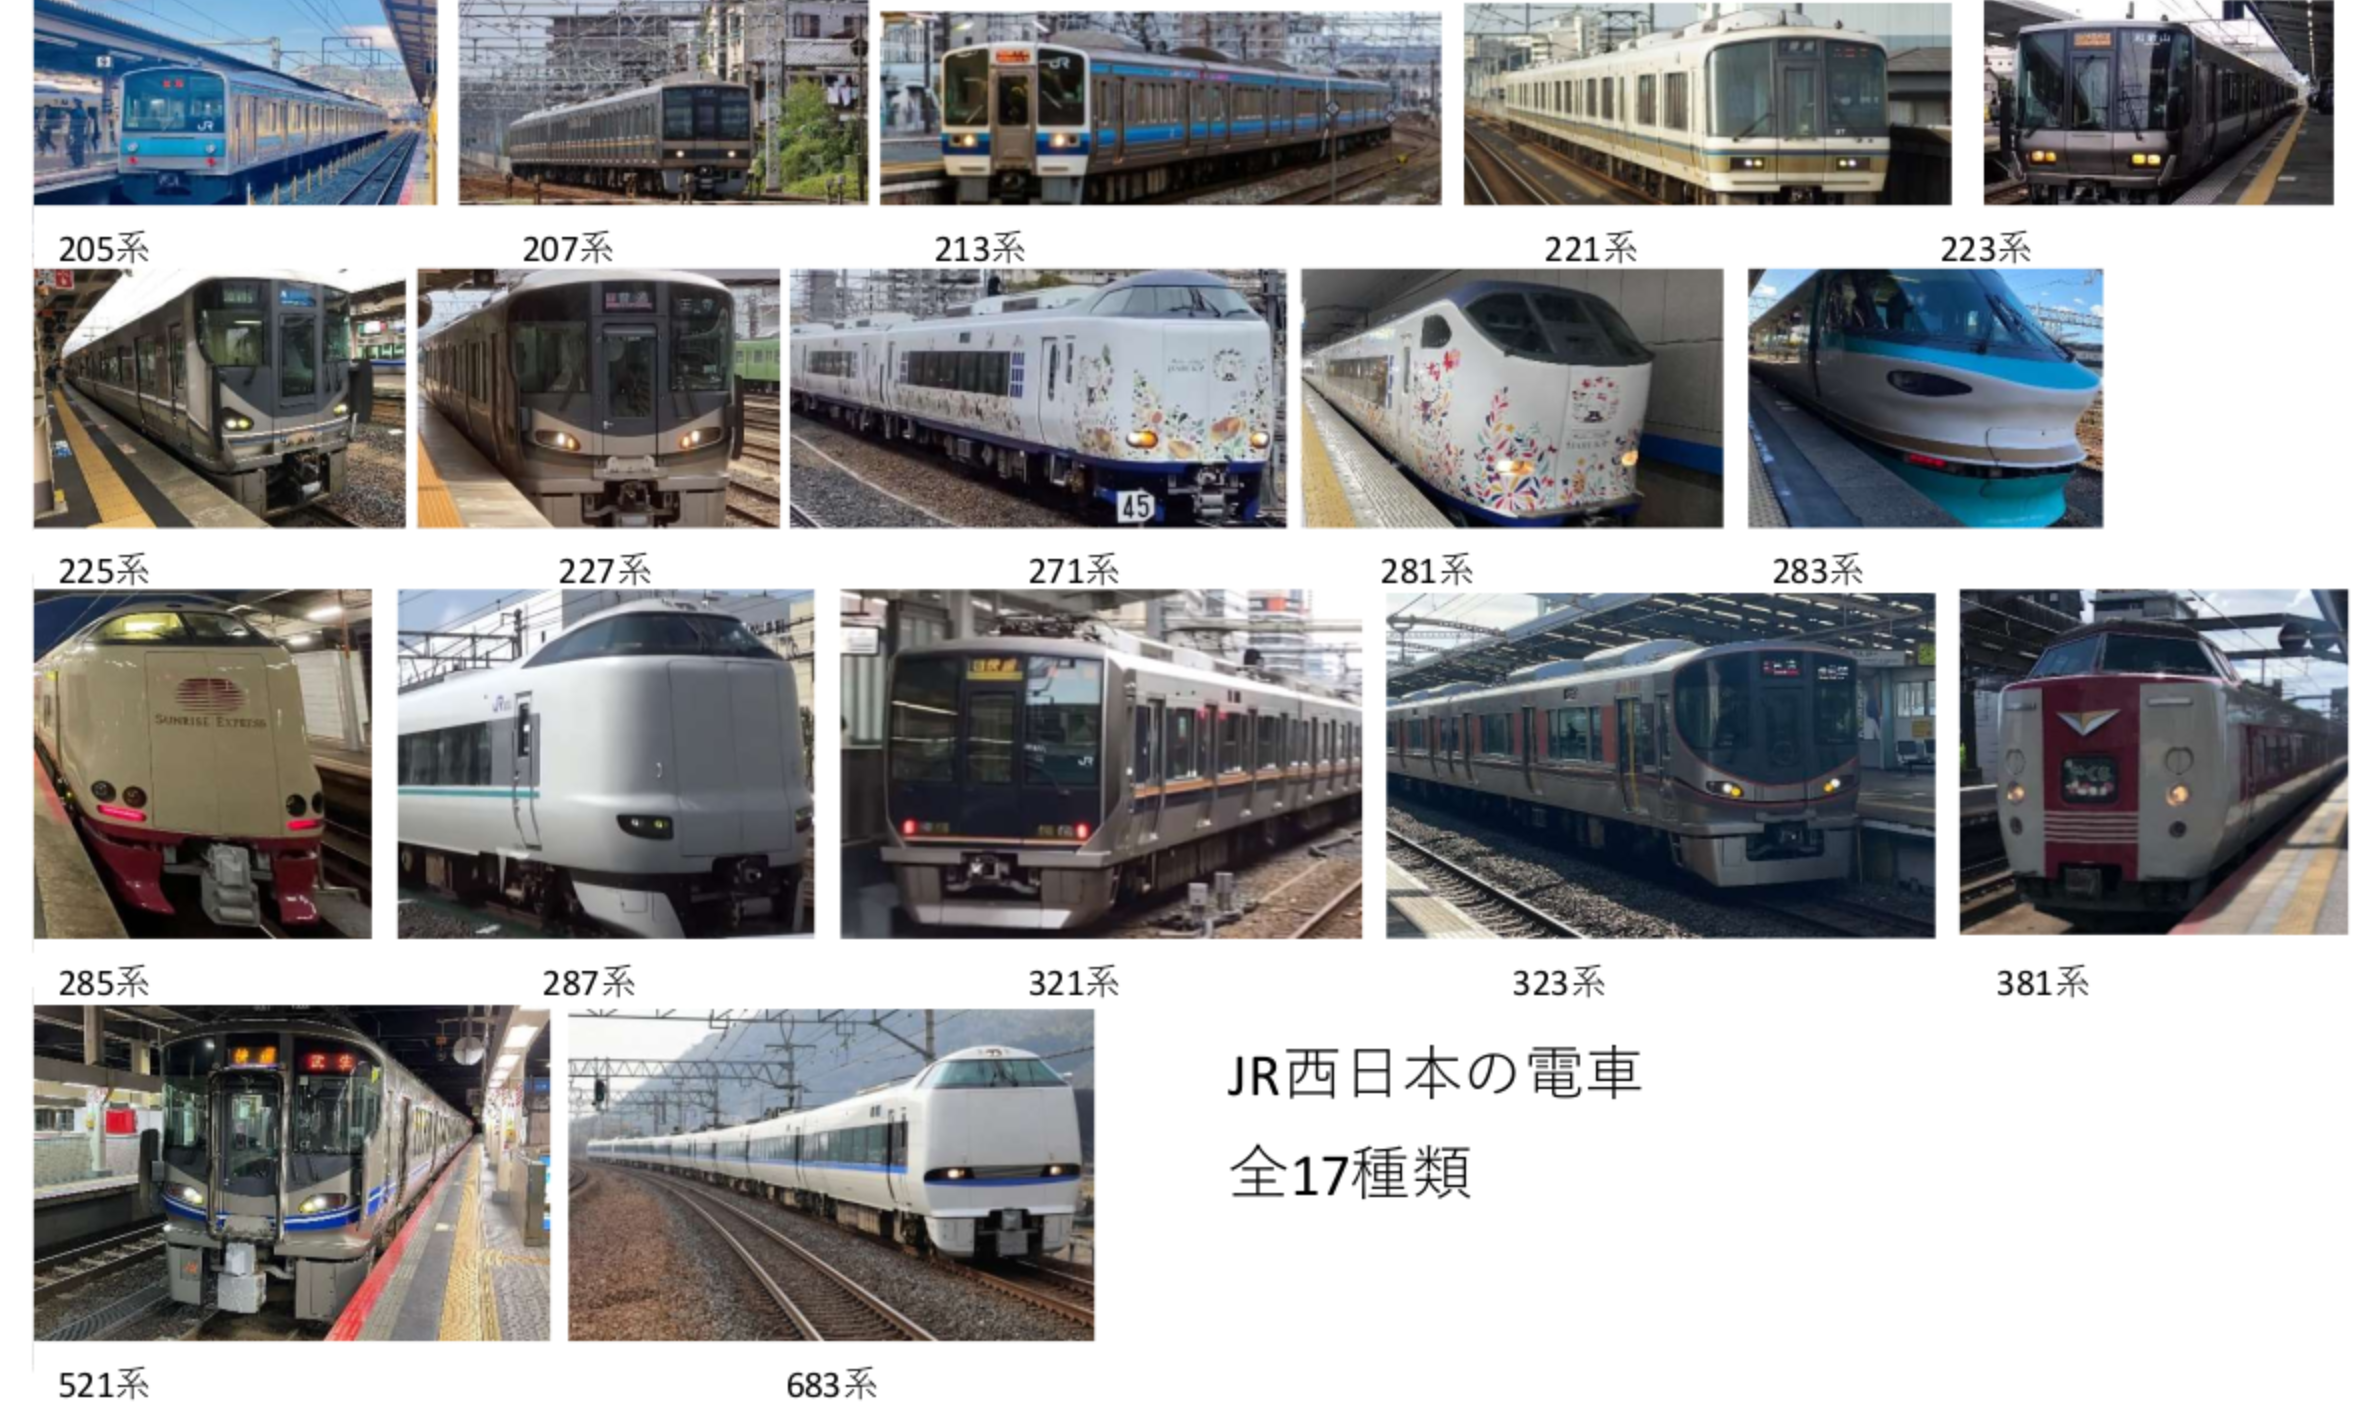
\includegraphics[width=0.6\linewidth]{fig/densya0202.png}
	\caption{車両タイプ一覧}
	\label{fig:densya0202}
\end{figure}





\foilhead{\Large 5-2.データセット作成の流れ}
\begin{enumerate}
	\item YouTubeから動画を保存する
	\item ランダムなフレームを5000枚保存する
	\item 電車が写っていないものを削除する
	\item  (識別用データセット作成時のみ)アノテーションをする
\end{enumerate}
各車両タイプごとに行い17種類の車両タイプのデータセットを作成した.

動画を効率的に保存するためのWebアプリを作成した.

\foilhead{\Large 5-3.動画を効率的に集めるWebアプリ}

\begin{itemize}
	\item 一つの動画に複数種類の電車が写っていると\\データセットをうまく作れない.
	\item 特定の車両タイプのみが写っている動画を集める必要がある.
	\item 特定の車両タイプのみが写っている場面を元の動画から\\切り抜きできれば良い.
\end{itemize}
	

\newpage

\begin{figure}[htbp]

			\centering
			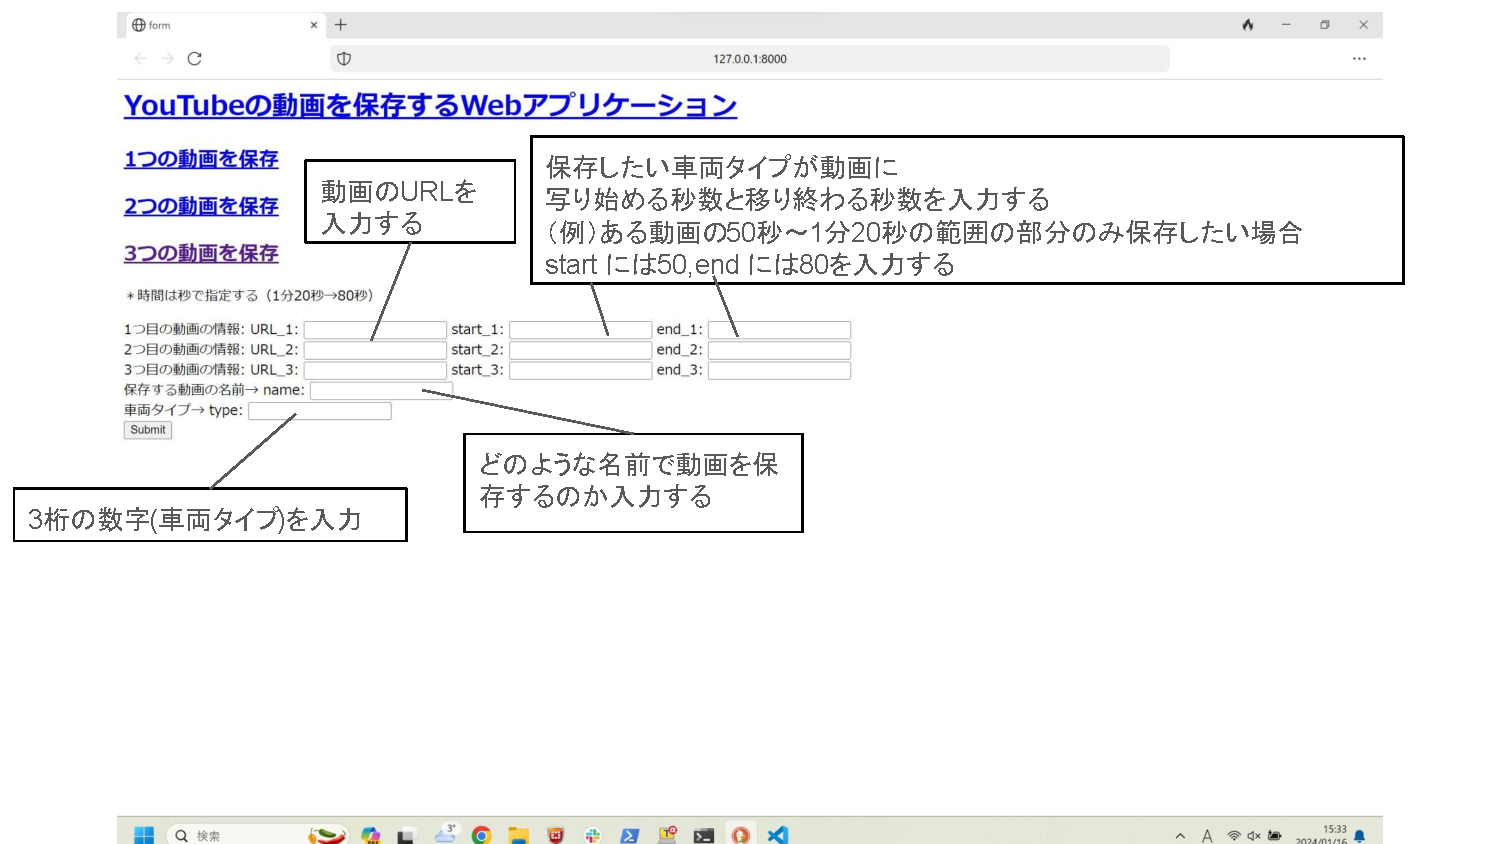
\includegraphics[width=0.75\linewidth]{../paper/chap3/fig/django}
			\label{fig:django}
			\caption{動画情報の入力画面}
			デモ動画\href{run:./fig/demo1.mp4}{\textcolor[hsb]{0.0, 0.7, 1.0}{\faPlayCircle[regular]}} 	

\end{figure}


%デモ動画\href{run:./fig/demo1.mp4}{\textcolor[hsb]{0.0, 0.7, 1.0}{\faPlayCircle[regular]}} 	

\newpage

車両タイプによって保存できた画像の枚数に差が生まれてしまった.

保存した画像は7:3の割合でトレーニングとバリデーションに分けた.
\begin{figure}
	\centering
	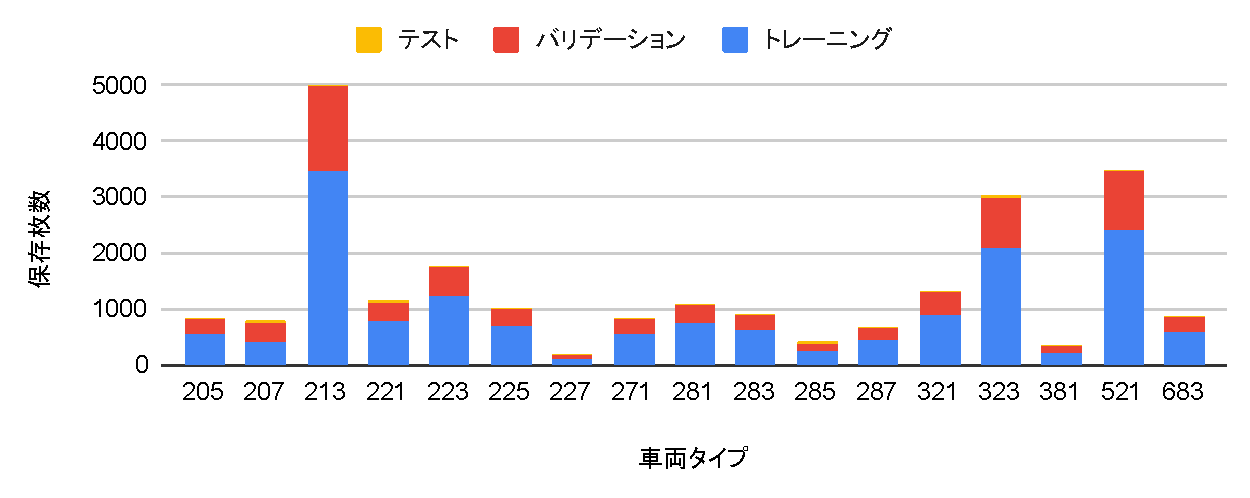
\includegraphics[width=0.8\linewidth]{fig/chart2}
	\caption{車両タイプ別の画像の保存枚数}
	\label{fig:chart2}
\end{figure}


\foilhead{\Large  6.モデルの作成 6-1.モデルの学習}
%分類モデルと識別モデルを学習させた.

\begin{figure}
	\centering
	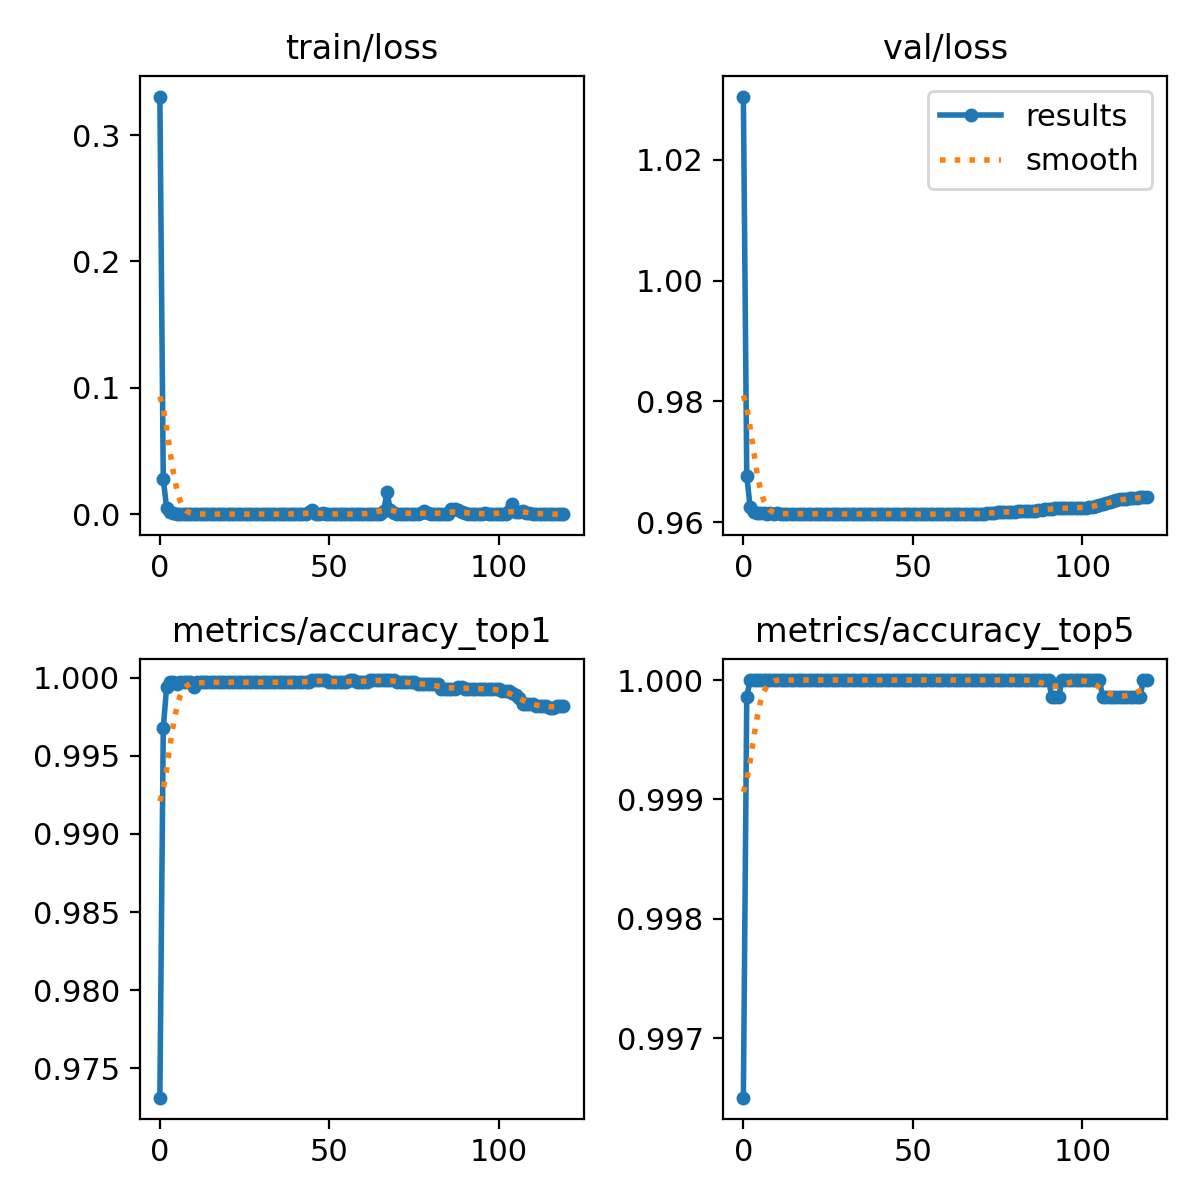
\includegraphics[width=0.65\linewidth]{fig/results_cls}
	\caption[分類モデルの学習曲線]{分類モデルの学習曲線}
	\label{fig:resultscls}
\end{figure}

\newpage

\begin{figure}
	\centering
	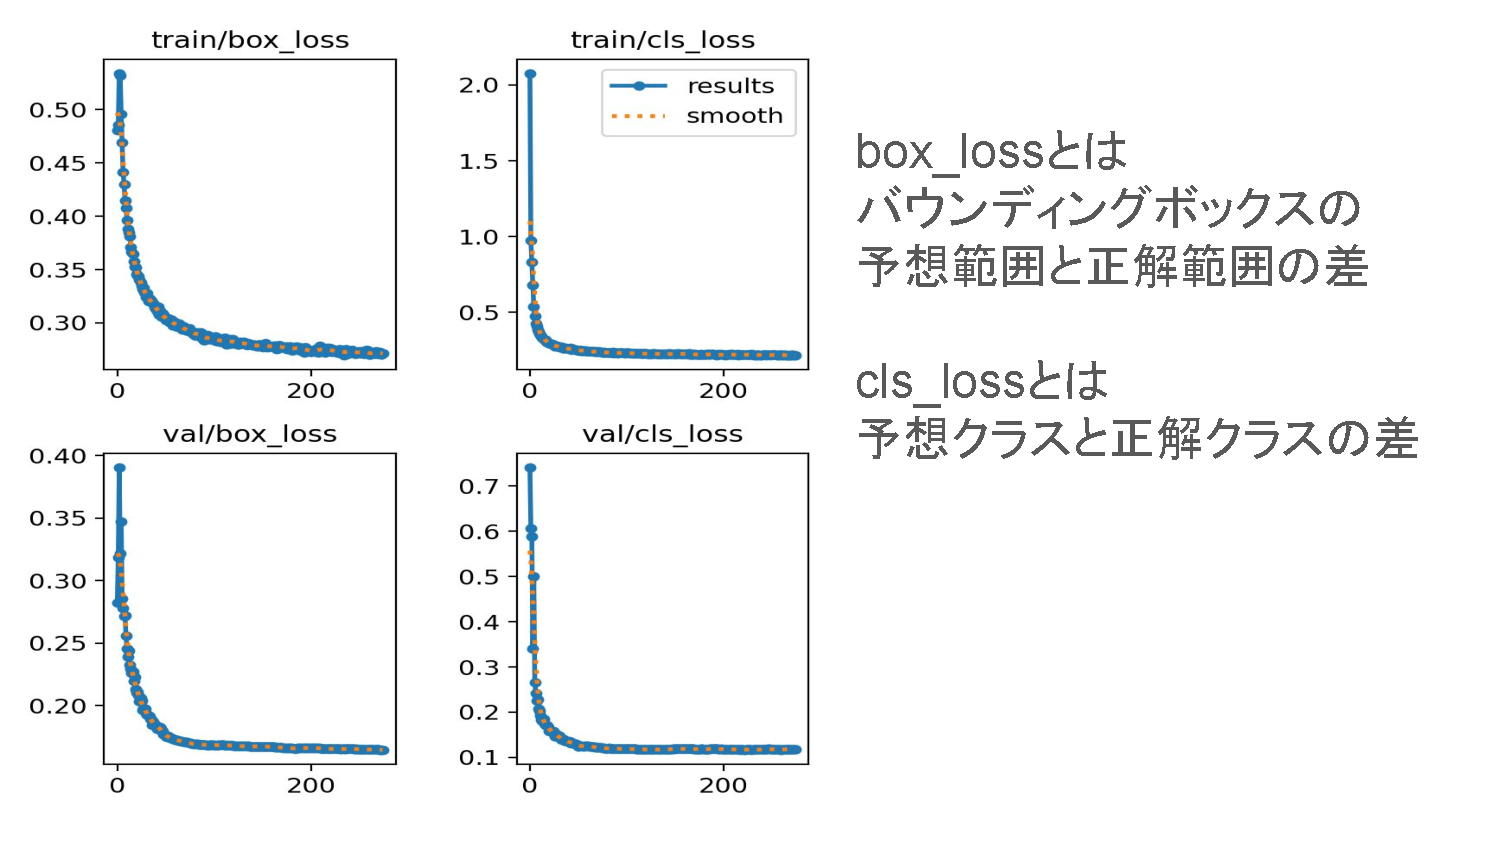
\includegraphics[width=0.8\linewidth]{fig/results_det}
	\caption[識別モデルの学習曲線]{識別モデルの学習曲線}
	\label{fig:resultsdet}
\end{figure}


\foilhead{\Large 6-2.作成したモデルの評価}
識別モデルと分類モデルは同様の方法で評価を行う.
\begin{itemize}
	\item 評価方法
	
	混同行列を作成する.
	
	テストデータセットを判別した際の正解数を測定する.
	
	

\end{itemize}
\newpage
\begin{figure}[htbp]
	\begin{minipage}[b]{0.5\linewidth}
		\centering
		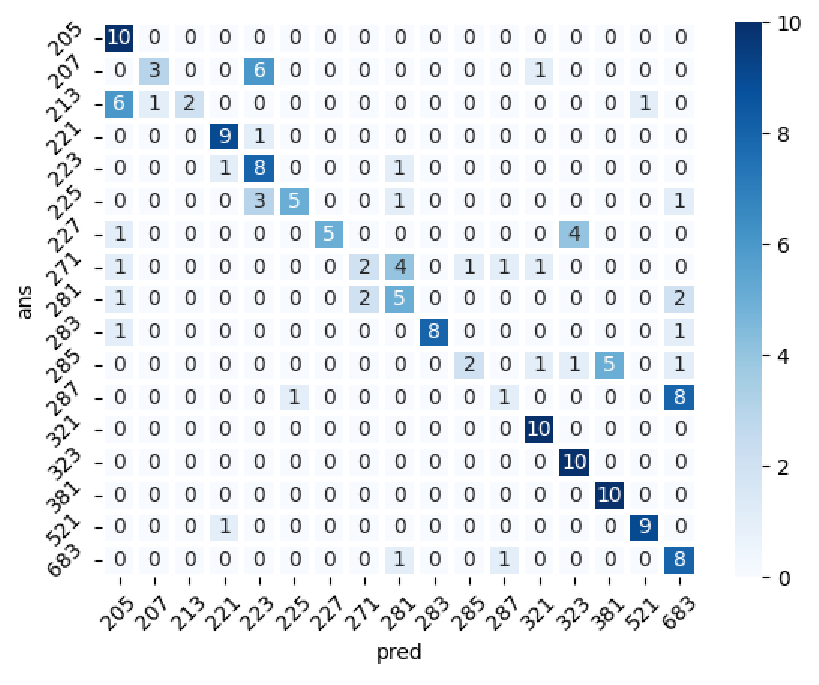
\includegraphics[width=\linewidth]{../paper/chap4/fig/classify_results}
		\caption{分類モデルの混同行列}
	\end{minipage}
  \begin{minipage}[b]{0.5\linewidth}
 	\centering
  	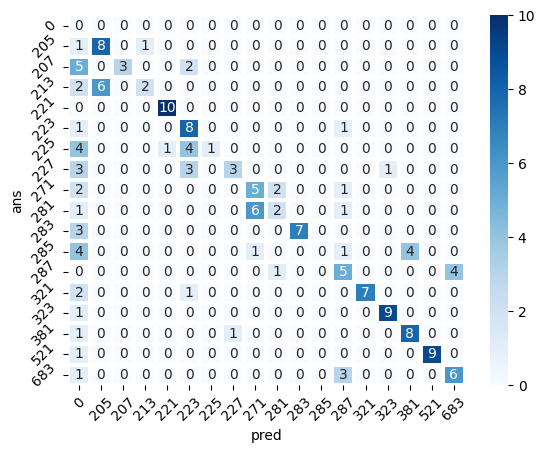
\includegraphics[width=\linewidth]{../paper/chap4/fig/predicted_results}
  	\caption{識別モデルの混同行列}
  	\label{det_confusion}
  \end{minipage}
\end{figure}



\newpage
\begin{figure}[htbp]
	\centering
	\begin{minipage}[b]{0.25\linewidth}
		\centering
		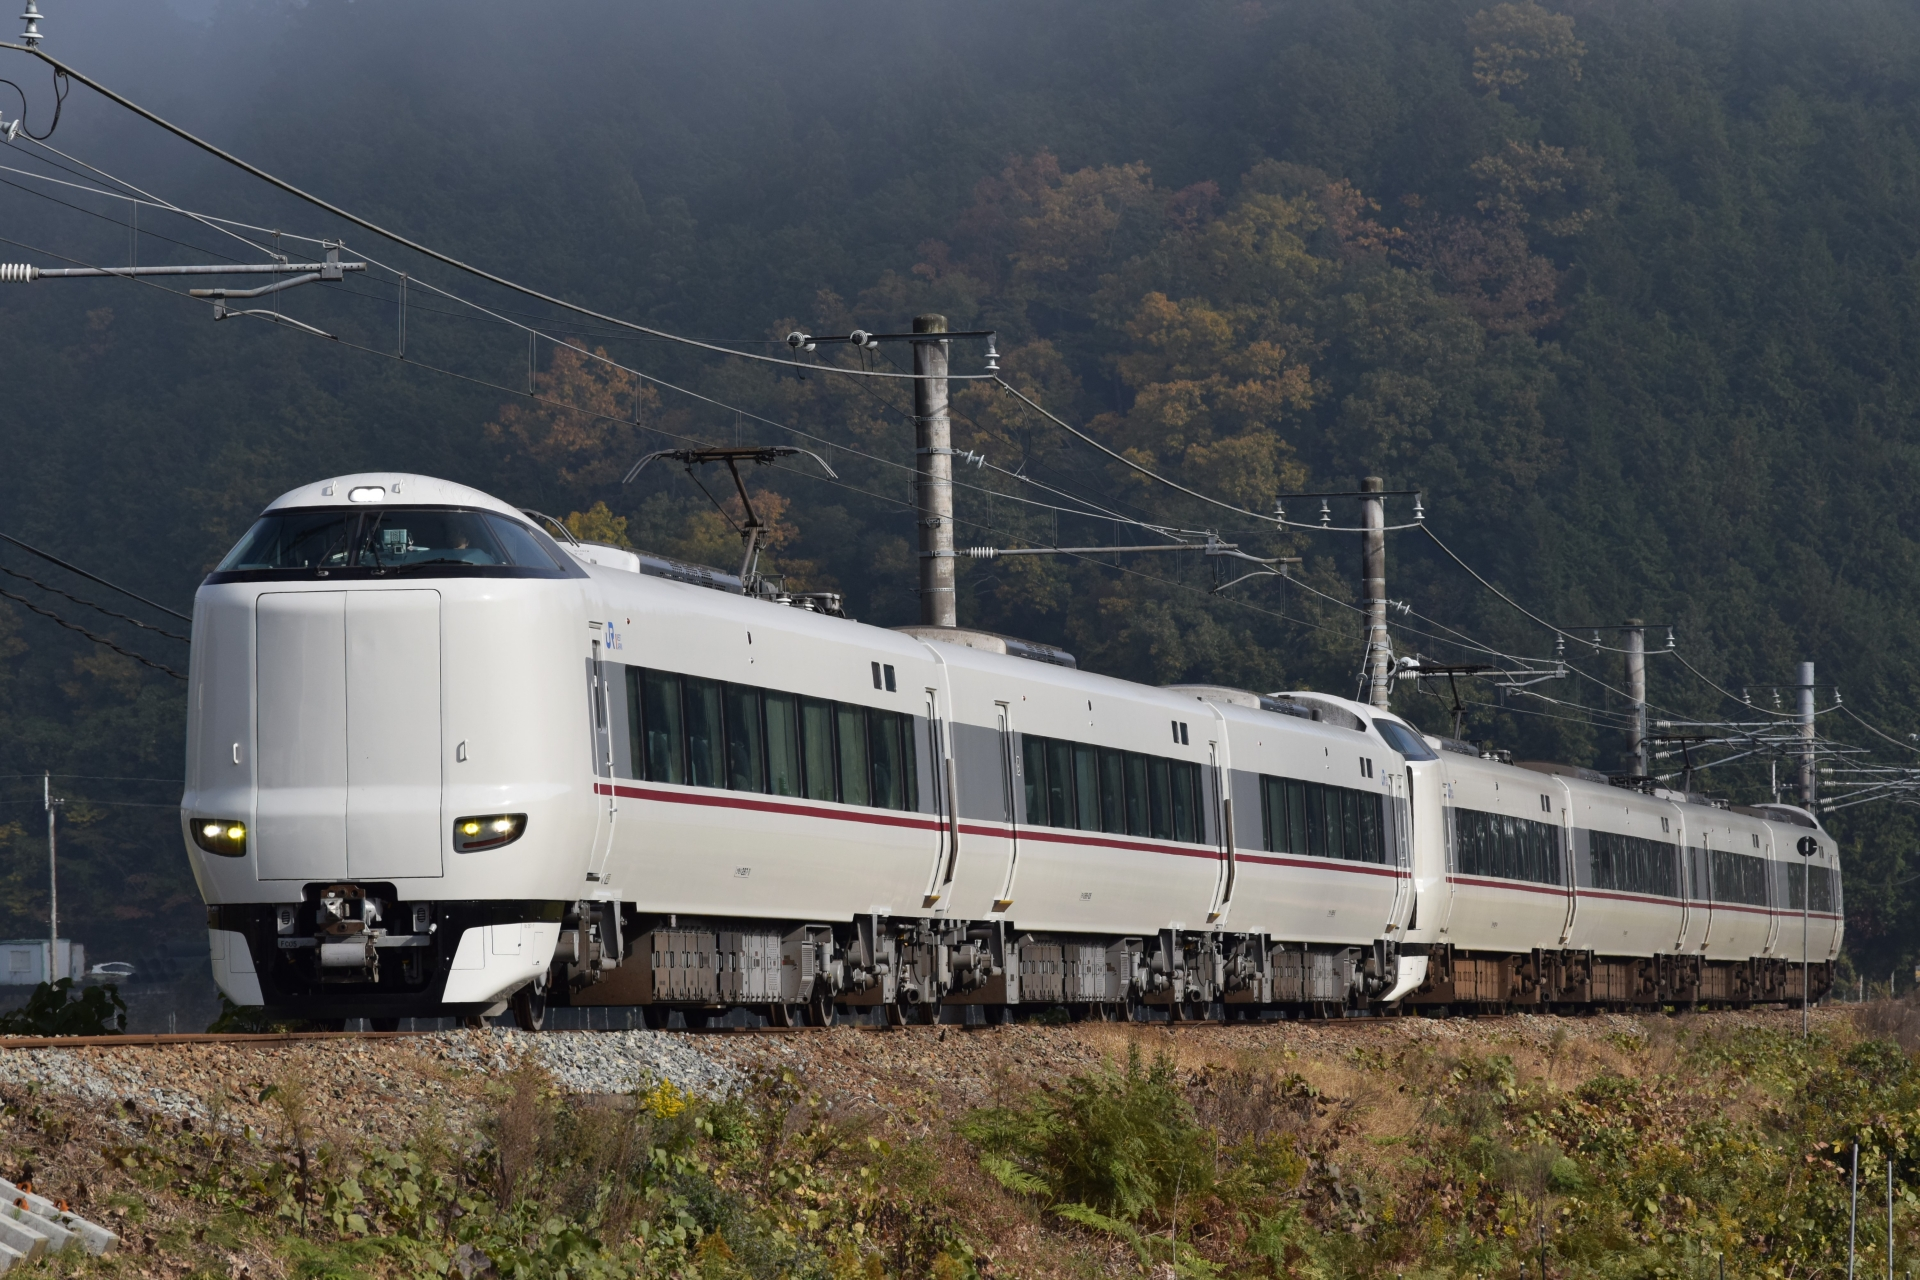
\includegraphics[width=\linewidth]{fig/287.jpg}
		\caption{287系}
		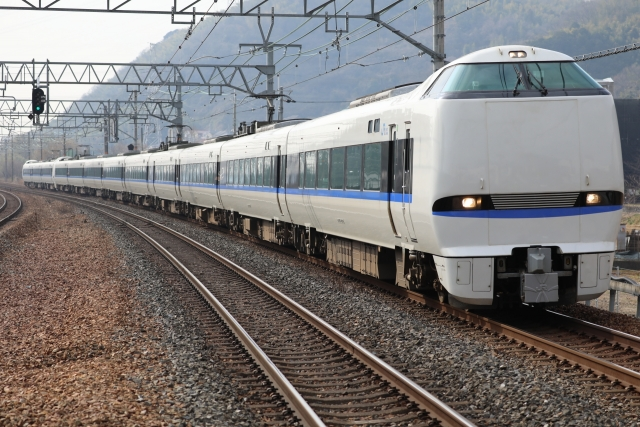
\includegraphics[width=\linewidth]{fig/683.jpg}
		\caption{683系}
	\end{minipage}
    \begin{minipage}[b]{0.5\linewidth}
		\centering
		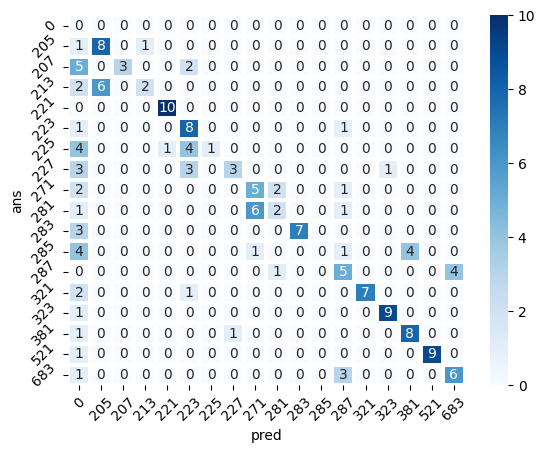
\includegraphics[width=\linewidth]{../paper/chap4/fig/predicted_results}
		\textbf{図 \ref{det_confusion} :識別モデルの混同行列}
	\end{minipage}
\end{figure}

\foilhead{\Large 6-3.モデルに関する考察}

 似た車両で誤判別が多かった.
 
 作成したデータセットに問題があると考えられる.
 
 改善案)

\begin{itemize}	
	\item 車両タイプごとの画像の枚数を揃える
	
	\item 電車の特徴が鮮明に写る画像を集める
	
	
\end{itemize}


\foilhead{\Large 7.むすび}

\begin{itemize}
	\item 動画を効率的に保存するためのWebアプリを開発した.
	\item 画像や動画に写る電車の車両タイプを判別するWebアプリを開発した.
	\item 一部の車両タイプは正確に判別できるようになった.
\end{itemize}


\begin{comment}
	

\begin{thebibliography}{99}
\small
\setlength\itemsep{-0.5\zh}%
\bibitem{book1} K.Thompson,D.M.Ritchie,\textbf{"The UNIX Time-Sharing System"},Communications of the ACM, Vol.17, No.7, 1974.
\bibitem{book4} Digital Equipment Corporation: \textbf{PDP11/20-15-r20 Processor Handbook}, 1971.
\bibitem{Preliminary} T.R. Bashkow, \textbf{"Study of UNIX: Preliminary Release of Unix Implementation Document"}, \url{ http://minnie.tuhs.org/Archive/Distributions/Research/Dennis_v1/PreliminaryUnixImplementationDocument_Jun72.pdf}, Jun. 1972.
%\bibitem{book2} K. Thompson,D.M. Ritchie,"UNIX PROGRAMER'S MANUAL",Nov. 1971.
%\bibitem{web0} Warren Toomey, "The Unix Heritage Society", \url{https://www.tuhs.org/}, Dec. 2015.
\bibitem{simh} simh, \textbf{"The Computer History Simulation Project"}, \url{https://github.com/simh/simh}, 参照Mar.14, 2022.
\bibitem{ref0} W.Toomey, \textbf{"First Edition Unix: Its Creation and Restoration"}, IEEE Annals of the History of Computing, 32 (3), pp.74-82, 2010.
%\bibitem{web1} Jim Huang, "Restoration of 1st Edition UNIX from Bell Laboratories", \url{https://github.com/jserv/unix-v1}, 参照Mar.14, 2022.
\bibitem{book3} Diomidis.Spinellis,\textbf{"unix-history-repo"},  \url{https://github.com/dspinellis/unix-history-repo/tree/Research-V1}, 参照Mar.14, 2022.
\bibitem{book5} Digital Equipment Copporation: \textbf{PDP11 Peripherals HandBook}, 1972.
%\bibitem{book6} \url{https://github.com/No000/unix-v1-utils}
%\bibitem{book7} \url{https://github.com/No000/UnixV1-SystemCallTracer}
%\end{thebibliography}
%\end{comment}

%\begin{comment}
\begin{thebibliography}{99}
\small
\setlength\itemsep{-0.5\zh}
\bibitem{book1} ultralytics,  \textbf{"yolov5"}, \url{https://github.com/ultralytics/yolov5},2023.9.18.
\bibitem{book1} ultralytics,  \textbf{"yolov8"}, \url{https://github.com/ultralytics/ultralytics}, 2023.9.18.
\end{thebibliography}
\end{comment}
\end{document} 





